%\subsection{Backgrounds at high \qsq}

In data at stripping level, events where the \db candidate originates upstream of the \Bd vertex are observed,
particularly at high \qsq, as shown in \Fig{fig:negtau:withmc}.
The origin of this background is from a $B\Bbar$ pair, where one decays into a \mumu pair, and the
other into a \kpi.
The \chisqip cuts placed on the muons and hadrons make it so that the efficiency of reconstructing a 2-body decay is greater for higher 2-particle masses at short $B$ lifetimes (simply due to the extra kick given to the child particles).
Since we require the \kpi pair have a \Kstar mass, then in the high \qsq region the di-muon mass is much bigger than the \Kstar mass.  This means that the efficiency is higher at shorter distances from the PV to select the di-muon pair than the \Kstar; therefore, in the case where the \Kstar and di-muons come from different $B$ decays, it's more likely that the di-muon pair is closer to the PV and so appears to have a negative $\tau$.
The converse should be true when the \kpi mass is large and the di-muon mass is small and we see this effect in the data when requiring
the $K\pi$  mass be large and the di-muon mass
consistent with a \Kstar ($|m(\mumu)-m^{PDG}(\Kstar)|<100\mev$; as shown in
\Fig{fig:negtau:2d}.

This background does not concern us as it will populate the local sidebands (it does not peak in
di-muon mass) and so will be subtracted automatically by our procedure.  Furthermore, we do not
expect significant contributions in the positive lifetime  region.  This is shown in
\Fig{fig:res:mxvtau} in the $B$ mass sidebands where this background is seen at negative $\tau$ but
no evidence is seen fof it at positive $\tau$.

%At high \qsq in the data sample, we observed a tail in the negative direction in the distribution
%of $\tau(\db)$.
%The extent of this tail in different \qsq regions can be seen in \Fig{fig:negtau:withmc}.
%This background is a kind of combinatorial background, it can be seen in the data for
%$m^\mathrm{meas}(\Bd)-m^\mathrm{PDG}(\Bd)>100\mev$ in the $m(\db), \tau(\db)$ plane in
%\Fig{fig:negtau:2d}.

%This background comes from dark boson candidates that originate from behind the vertex of the \Bd,
%this happens because the $\chisq_\mathrm{IP}$ for high \qsq candidates is necessarily higher than
%that of a low \qsq candidate.
%Therefore these candidates are accepted.
%We tested this using the same decay with the mass criteria flipped, that is:
%\begin{itemize}
  %\item $m(\Kp\pim)$ is unrestrained (though interested in high mass),
  %\item $m(\mumu)\in[796,996]$ so as to mimic the \Kstar mass,
%\end{itemize}
%and looking at mass against lifetime the same effect is visible (though to a much lesser extent).




%\begin{figure}
  %\begin{center}
    %\subfloat[\label{fig:negtau:withmc:low}]{\includegraphics[width=0.48\textwidth]{anaNegTau_2_6}}
    %\subfloat[\label{fig:negtau:withmc:mid}]{\includegraphics[width=0.48\textwidth]{anaNegTau_6_15}}\\
    %\subfloat[\label{fig:negtau:withmc:high}]{\includegraphics[width=0.48\textwidth]{anaNegTau_15_20}}
  %\end{center}
  %\caption{\small
    %Lifetime distributions for $\tau(\db)<0$ for three \qsq regions:
    %\protect\subref{fig:negtau:withmc:low} $2<\qsq<6$,
    %\protect\subref{fig:negtau:withmc:mid} $6<\qsq<15$, and
    %\protect\subref{fig:negtau:withmc:high} $15<\qsq<20\gevgev$.
    %The double Gaussian PDF centred at zero is from a fit to a MC sample in the given \qsq range.
    %One can clearly see that a tail extending out towards negative lifetimes as \qsq increases.
  %}
  %\label{fig:negtau:withmc}
%\end{figure}


%\begin{figure}
  %\begin{center}
    %\includegraphics[width=0.48\textwidth]{anaNegTau_kpi_2d}
  %\end{center}
  %\caption{\small
    %Mass against its lifetime for \Kstar candidate.
    %A slight negative skew in the lifetime dimension is observed.
  %}
  %\label{fig:negtau:2d}
%\end{figure}





\subsubsection{Backgrounds from particle misidentification}
\label{sec:db:backgrounds:misid}
A possible source of contamination comes from particles which are incorrectly identified as the
$\Kstarz\mumu$ final state.
A meson that decays via $\decay{X}{hh^\prime}$ which is then reconstructed
under the incorrect mass hypothesis could pass the selection criteria.
This type of contamination is studied by assigning different mass hypotheses to each final state
particle and calculating the invariant mass of the \mumu and \kpi candidates.
If the mass of one of these objects is seen to peak at the mass of a known particle, then the
contamination is removed  by applying \pid criteria to particles whose reassigned invariant mass
falls near $\mass{X}$.

Since a selection has been made on the \decay{\Kstarz}{\kpi} candidate using both \pid criteria and
constraints on the \kpi invariant mass it is expected that there will be little contamination
from background sources.
In order to be sure, \Kstarz candidates which come from a \Bd candidate which has an invariant mass
within $80\mev$ of the known \Bd mass are given different mass hypotheses to check for peaking
components in the new $\mass{K_{h}^+\pi_{h^\prime}^-}$ mass spectrum\footnote{
  Where, as defined previously, the notation $h_i$ is a particle under the mass hypothesis of $h$
  which was reconstructed as an $i$.
}.
The only background that must be removed from this category is from a real \decay{\phi}{\kk}
where a kaon in the final state is misidentified as being a pion.
If the mass of the $\Kp K^-_\pi$ candidate lies within $10\mev$ of the known \phii mass, the
ambiguous pion is subject to the requirements that
$\ProbNN{\pi}<0.3$ and $\ProbNN{K}>0.3$.

Backgrounds from resonances decaying into a pair of hadrons which are then mistaken as a pair of
hadrons are more problematic.
Misidentification of the decay \decay{\KS}{\pipi} is already dealt with in the preslection, but
there is also contamination from other long-lived hadronic states, namely the \Dz and \Lz.
The decays \decay{\Dz}{\kpi} and \decay{\Lz}{p\pim} are dealt with in a simiar way to the vetoes
described in \Sec{sec:dsphi:sel:veto}.
If the invariant mass of the $K^+_\mu\pi^-_\mu(p_\mu\pi^-_\mu)$ candidate falls within $25(10)\mev$
of the nominal $\Dz(\Lz)$ mass, then the ambiguous muon is subject to the requirement that
$\ProbNN{\mu}>0.3(\ProbNN{p}<0.3)$.


\begin{table}
  \caption[Double misidentification vetoes]
  {
   Vetoes from double and single misidentification of particles.
   If, under the alternate hypothesis, the \db or \Kstarz candidate mass falls within the range
   indicated under, the candidates are subject to the given \pid requirements.
  }
  \label{tab:bkg:vetoes}
  \begin{center}
    \begin{tabular}{lcc}\toprule
      \multicolumn{2}{c}{Mass criteria (MeV)} & PID requirement \\\midrule
      $\left|m(\Kp K^-_\pi) - m^\mathrm{PDG}_\phi\right|$ & $<10$
      & $\ProbNN{pi}(\pi)>0.3$ and \ProbNN{K}$(\pi)<0.3$
      \\\rule{0pt}{3ex}$\left|m(K^+_\mu\pi^-_\mu) - m^\mathrm{PDG}_{\Dz}\right|$& $<25$
      & $\ProbNN{mu}(\mu)>0.3$
      \\\rule{0pt}{3ex}$\left|m(p_\mu\pi^-_\mu) - m^\mathrm{PDG}_{\Lz}\right|$ & $<10$
      & $\ProbNN{p}(\mu)<0.3$  \\
      \bottomrule
    \end{tabular}
  \end{center}
\end{table}

There are also contributions from the decay \decay{\Bd}{\jpsi\Kstarz} and \decay{\jpsi}{\mumu},
where one of the hadron is misidentified as a muon, and vice versa.
This can be trivially removed by requiring that the hadrons do not satisfy {\tt isMuon}, as shown
in \Fig{fig:bkg:doublemisid}.

%\begin{figure}
  %\begin{center}
    %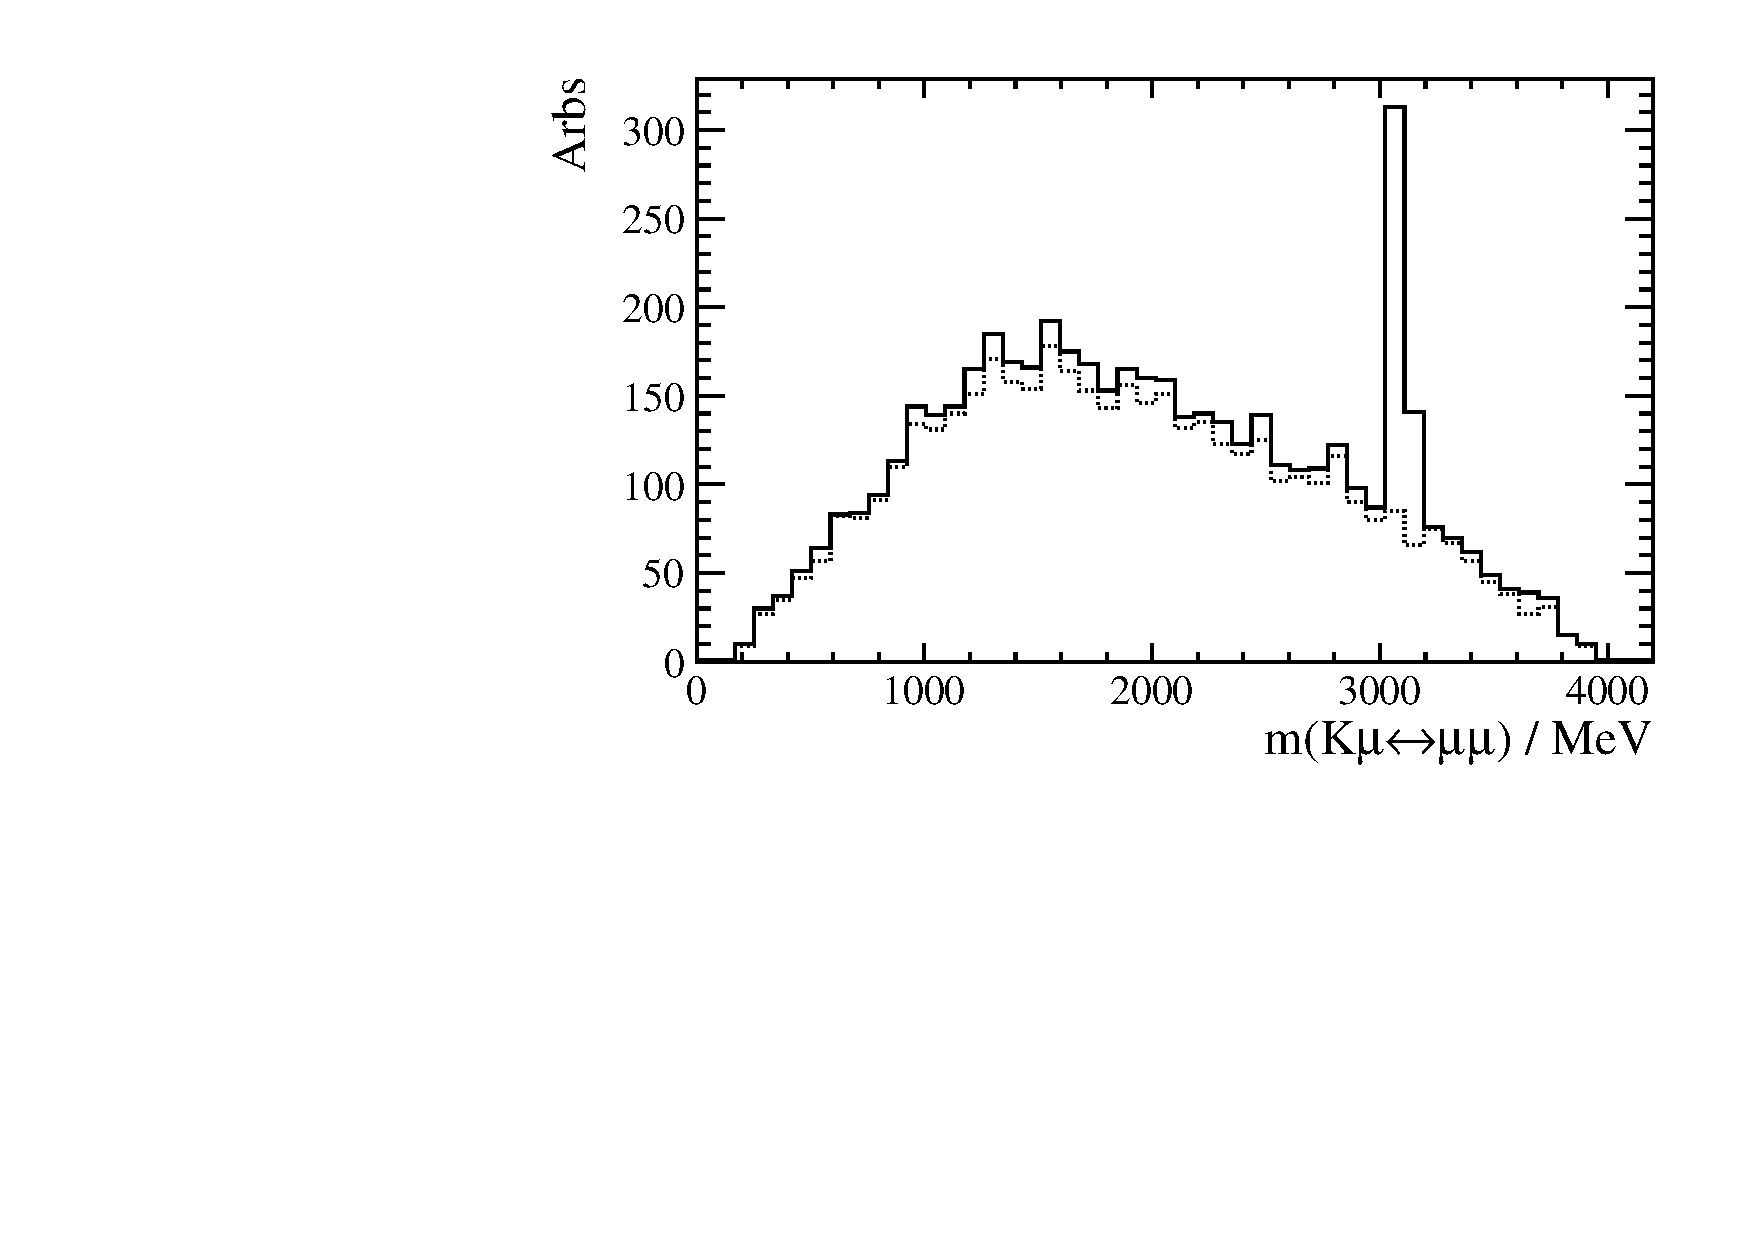
\includegraphics[width=0.48\textwidth]{double_misid_pi}
    %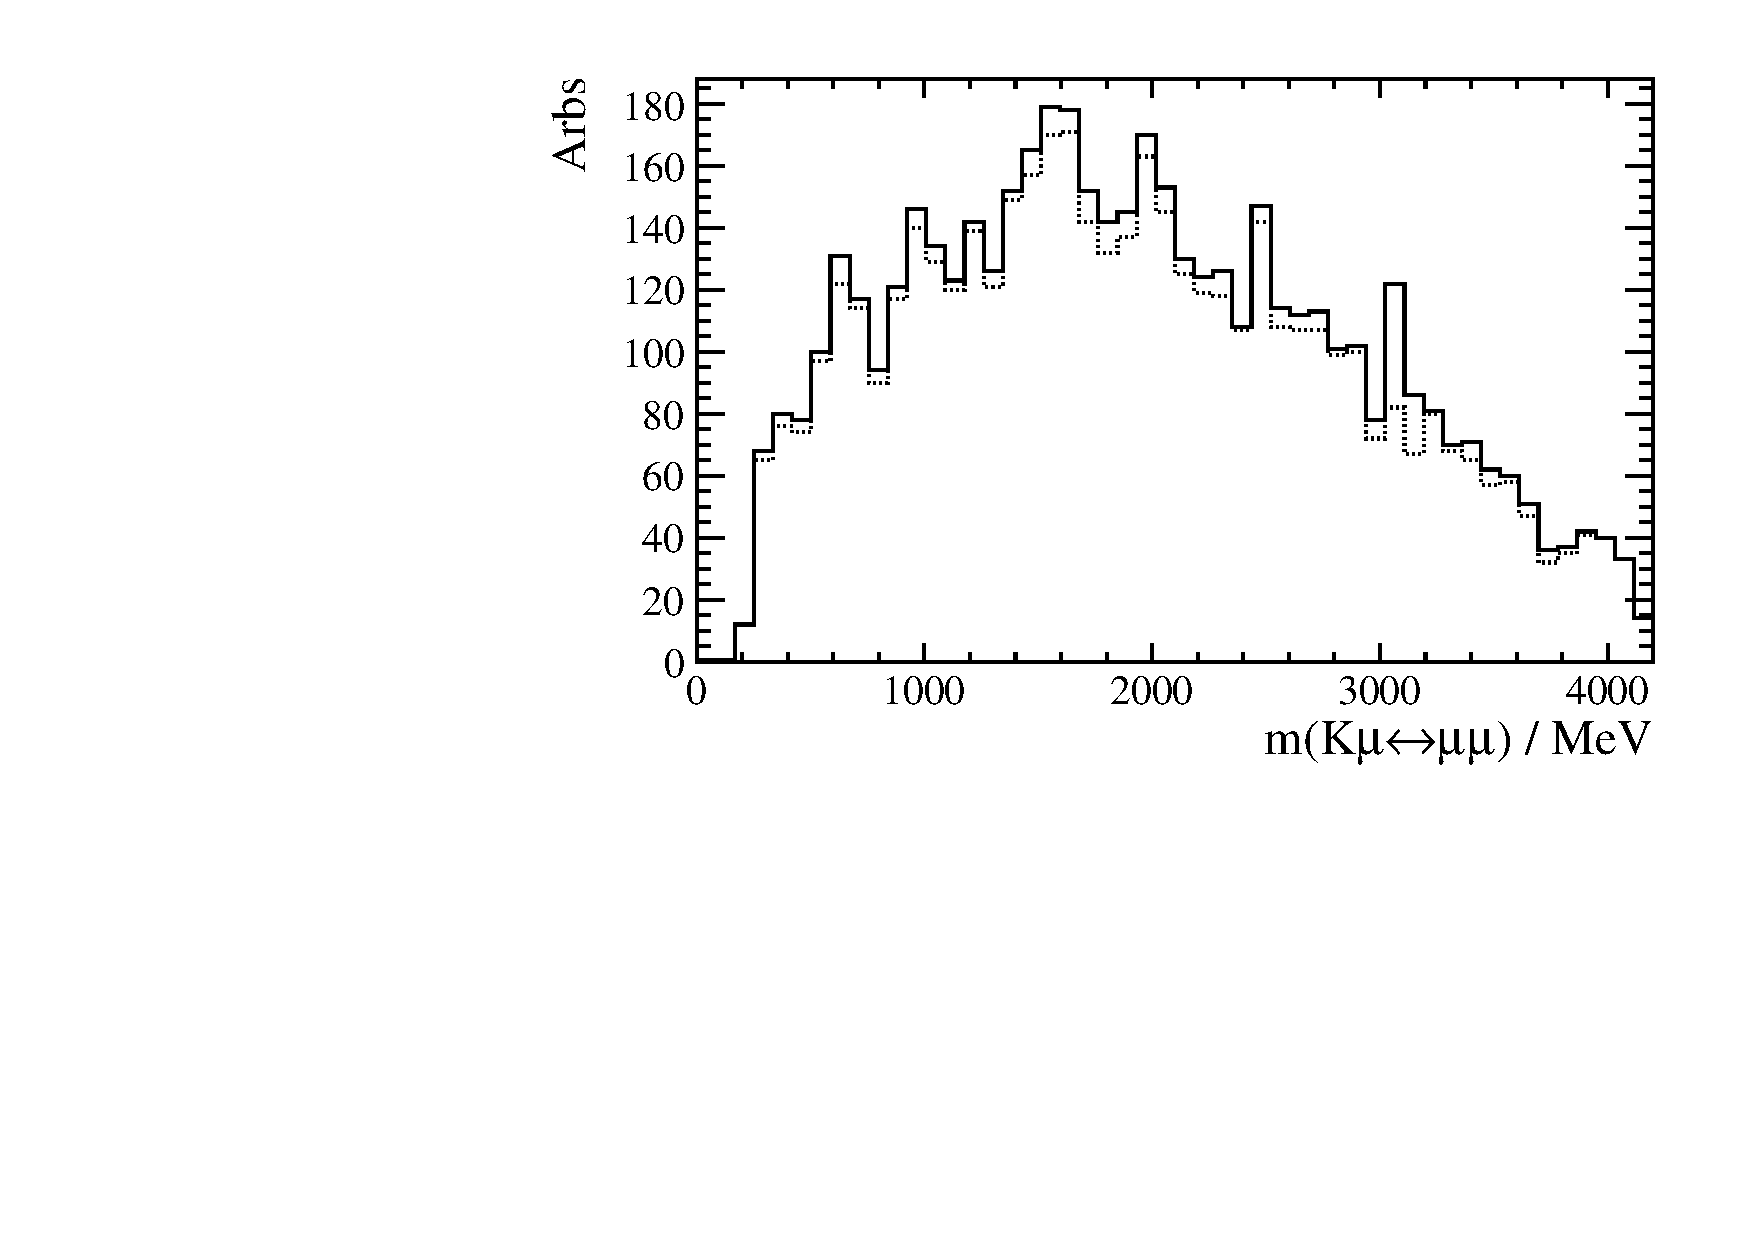
\includegraphics[width=0.48\textwidth]{double_misid_k}
    %\caption{\small
      %Background contributions from \decay{\Bd}{\jpsi\Kstarz}, where both a muon and (left) pion
      %and (right) kaon are misidentified as one another.
      %This background is very effectively removed by requiring that the hadron does not satisfy the
      %{\tt isMuon} criteria; the effect of this veto is shown with a dotted line.
    %}
    %\label{fig:bkg:doublemisid}
  %\end{center}
%\end{figure}

The sidebands are used to estimate the level of background in the signal region, and therefore
background
contributions are only problematic if they produce a narrow peaking structure in the dimuon mass.
Since misidentification results in smearing out of the mass, in general misidentification can only
cause a problem if the decaying particle has a very narrow natural width.
Therefore, any remaining misidentification-type backgrounds have negligible effect in the analysis.



\subsubsection[The \xtsvty]{The $\boldsymbol{\xtsvty}$}
\label{sec:x1070}

While searching for potential backgrounds resulting from misidentifying two hadrons as muons, a
peak was found in the invariant mass spectrum of the $K_\mu^+K_\mu^-$ candidates.
This peak was consistent with the \xtsvty listed in Ref.~\cite{PDG2014}, which has a mass of
$(1072\pm1)\mev$ with a width of $(3.5\pm0.5)\mev$ and was observed in the $\KS\KS$ distribution
from $\pim p \to \KS \KS n m\piz$ collisions~\cite{x1070vlad}, where $m\in\mathbb{Z}$.
Figure~\ref{fig:x1070} shows the observation of this resonance from \Ref{x1070vlad} alongside
the data from this analysis.

\begin{figure}
  \begin{center}
    %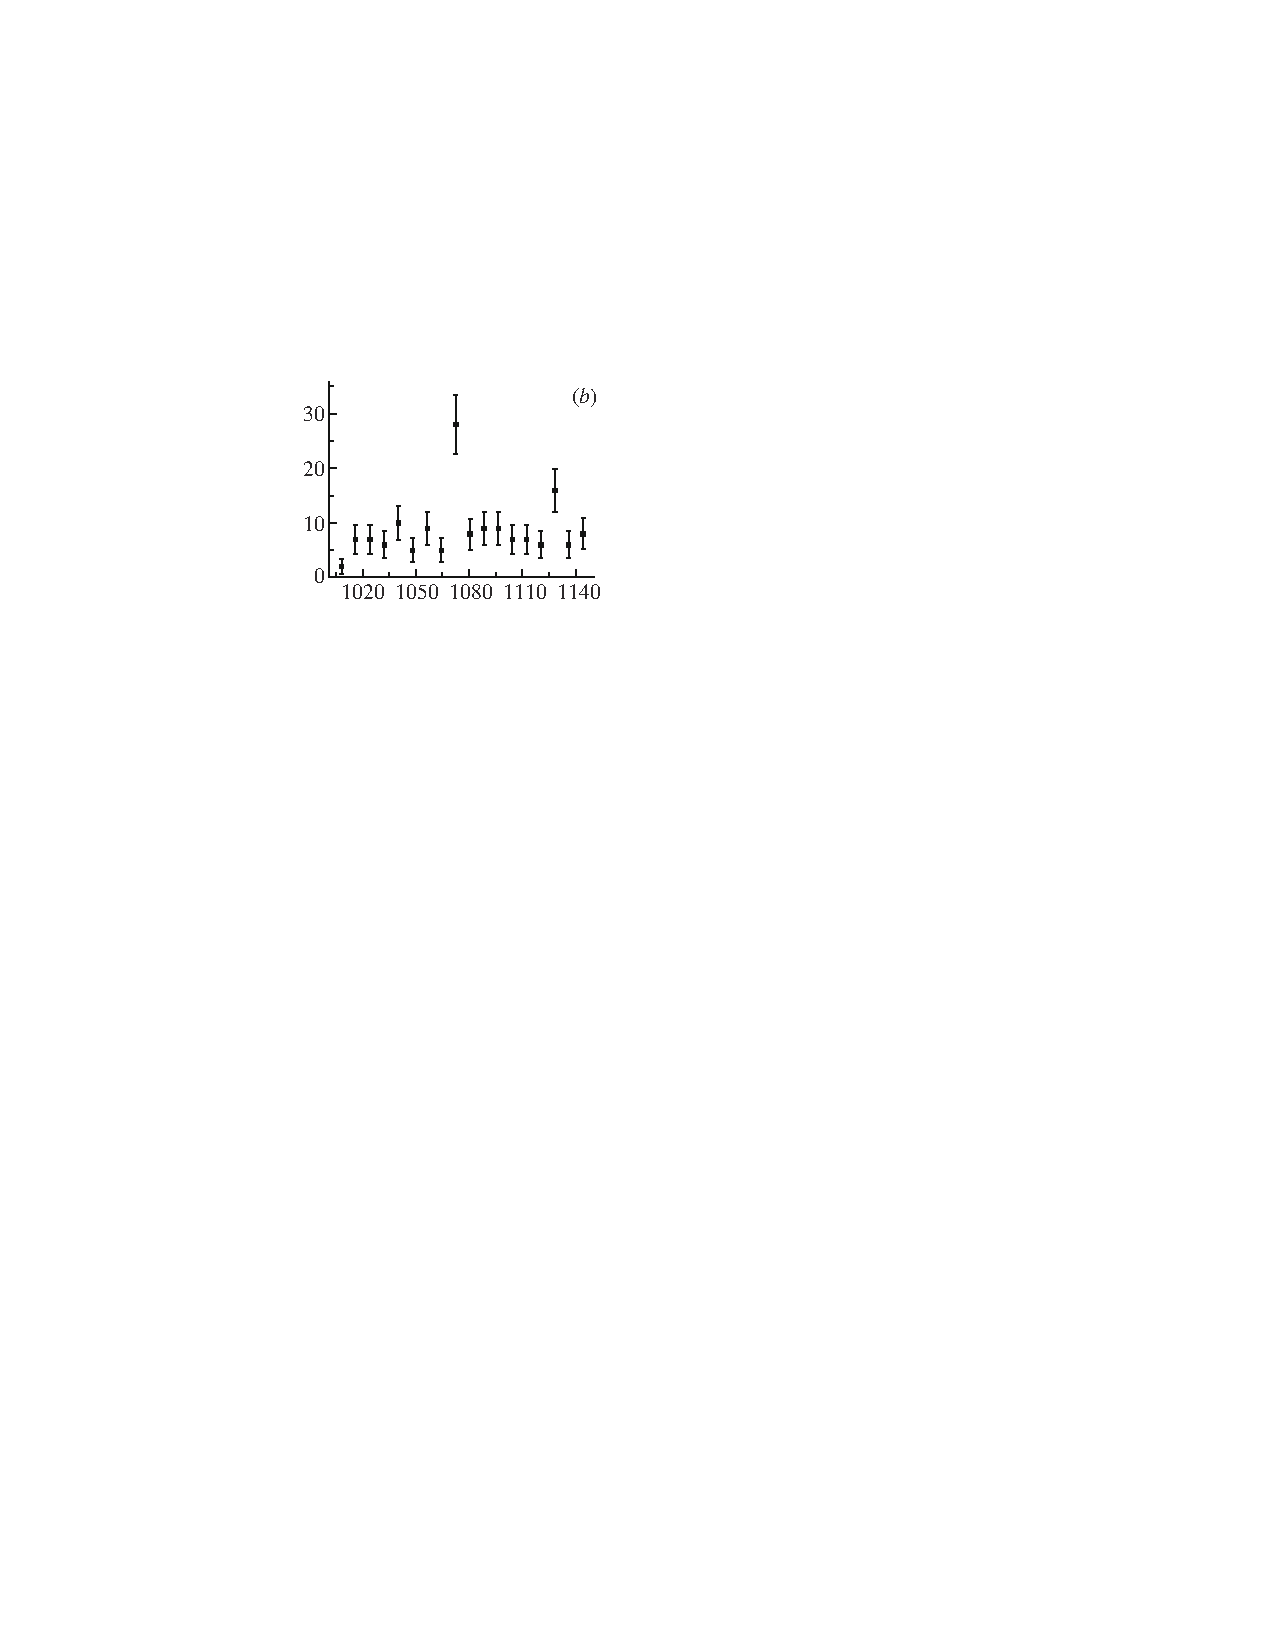
\includegraphics[height=0.2\textheight]{x1070vlad}
    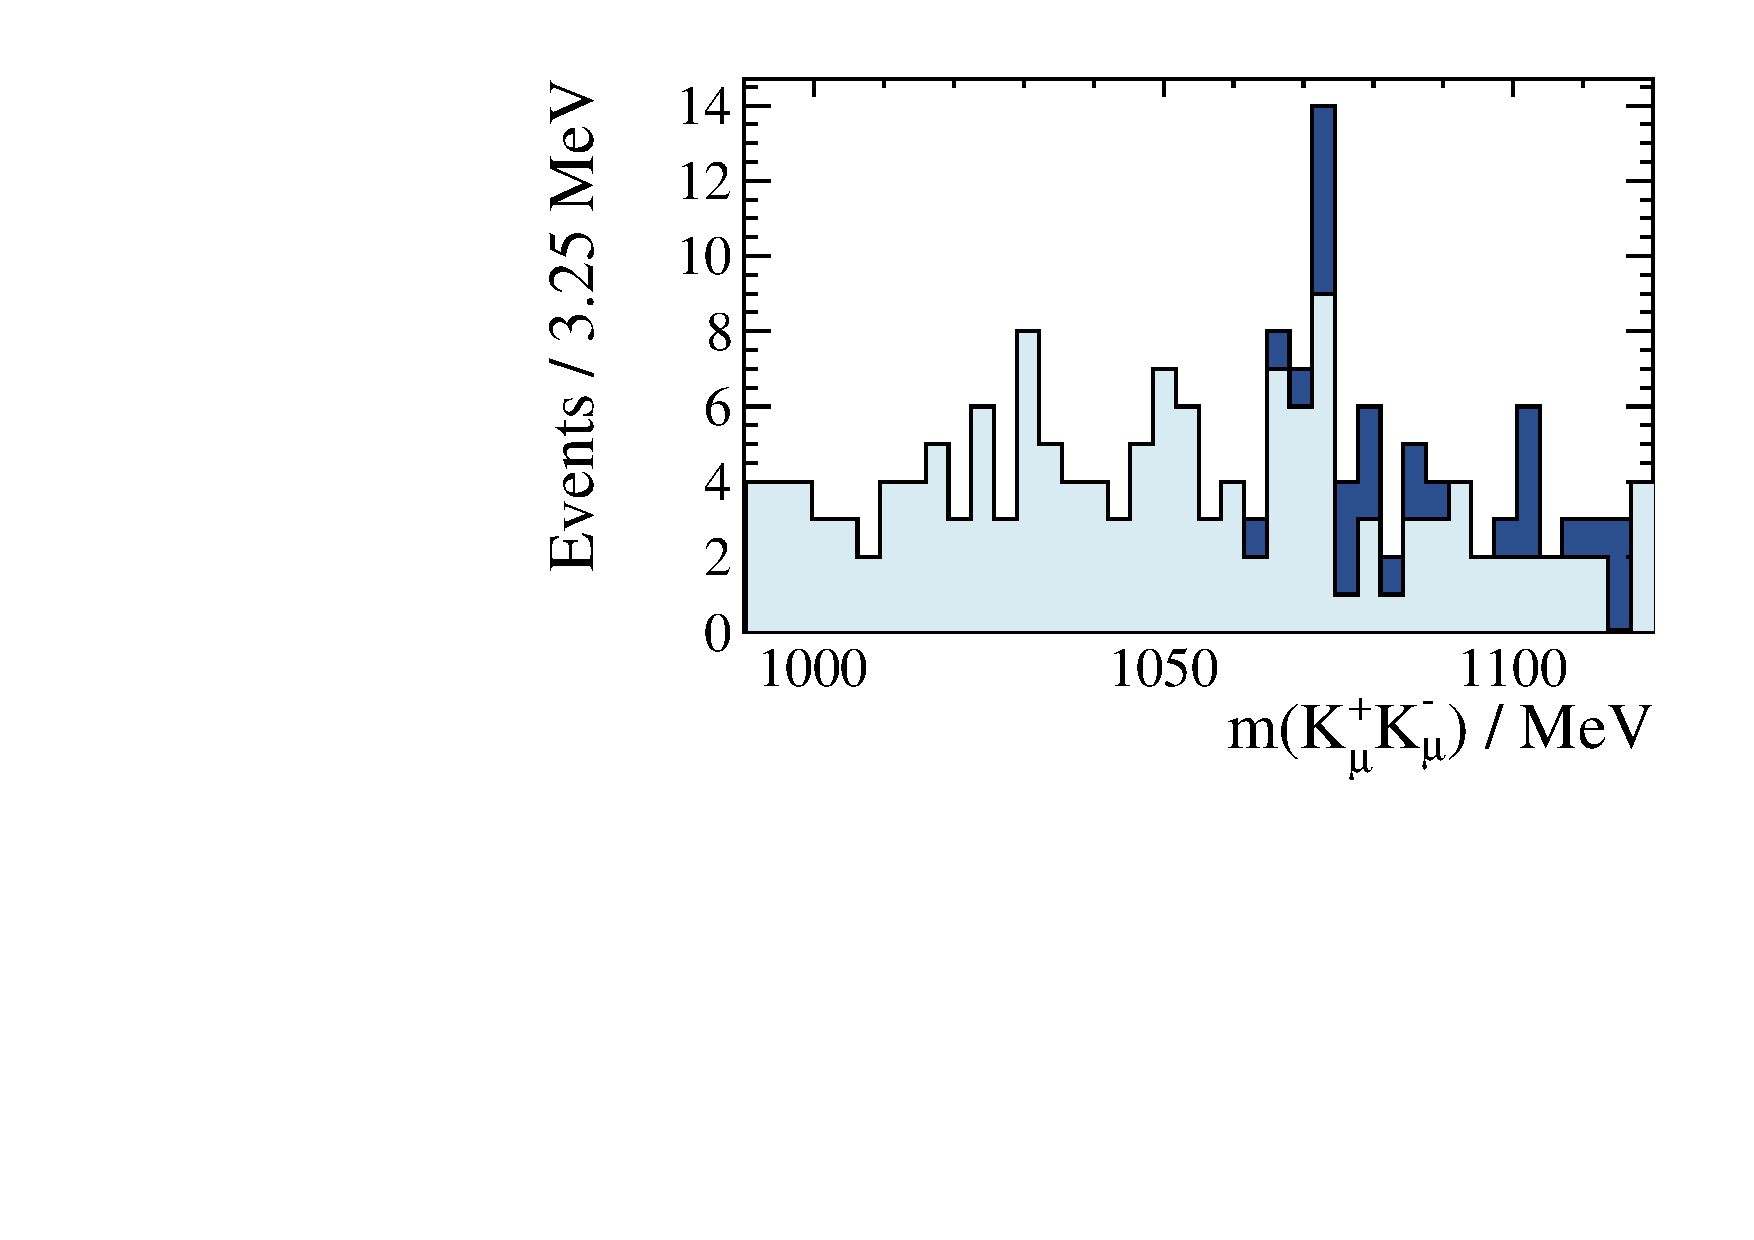
\includegraphics[height=0.2\textheight]{mumu_kk}
    \caption[Invariant mass of the \mumu distribution under the \kk mass hypotheses]
    {
      %A comparison of
      %(left) the data which observes the \xtsvty~\protect\cite{x1070vlad}, and
      Invariant mass distribution of the $K_\mu^+K_\mu^-$ candidates in data, showing a peak at
      \approx$1072\mev$ in data.
      The dashed line indicates the effect of vetoing the decay
      \decay{\KS}{\pip\pim} in the preseletcion.
    }
    \label{fig:x1070}
  \end{center}
\end{figure}

Figure~\ref{fig:db:x1070:2d} shows a comparison of simulated \decay{\KS}{\pipi} decays with the
observed data near this excess.
It is clear that \decay{\KS}{\pipi} decays produce a peak around $1070\mev$ under the \kk
hypothesis.
There is also a long tail but with low statistics and with a roughly uniform
background this tail would not be expected to be visible in the data after the \KS veto in the
preselection.

\begin{figure}
  \begin{center}
    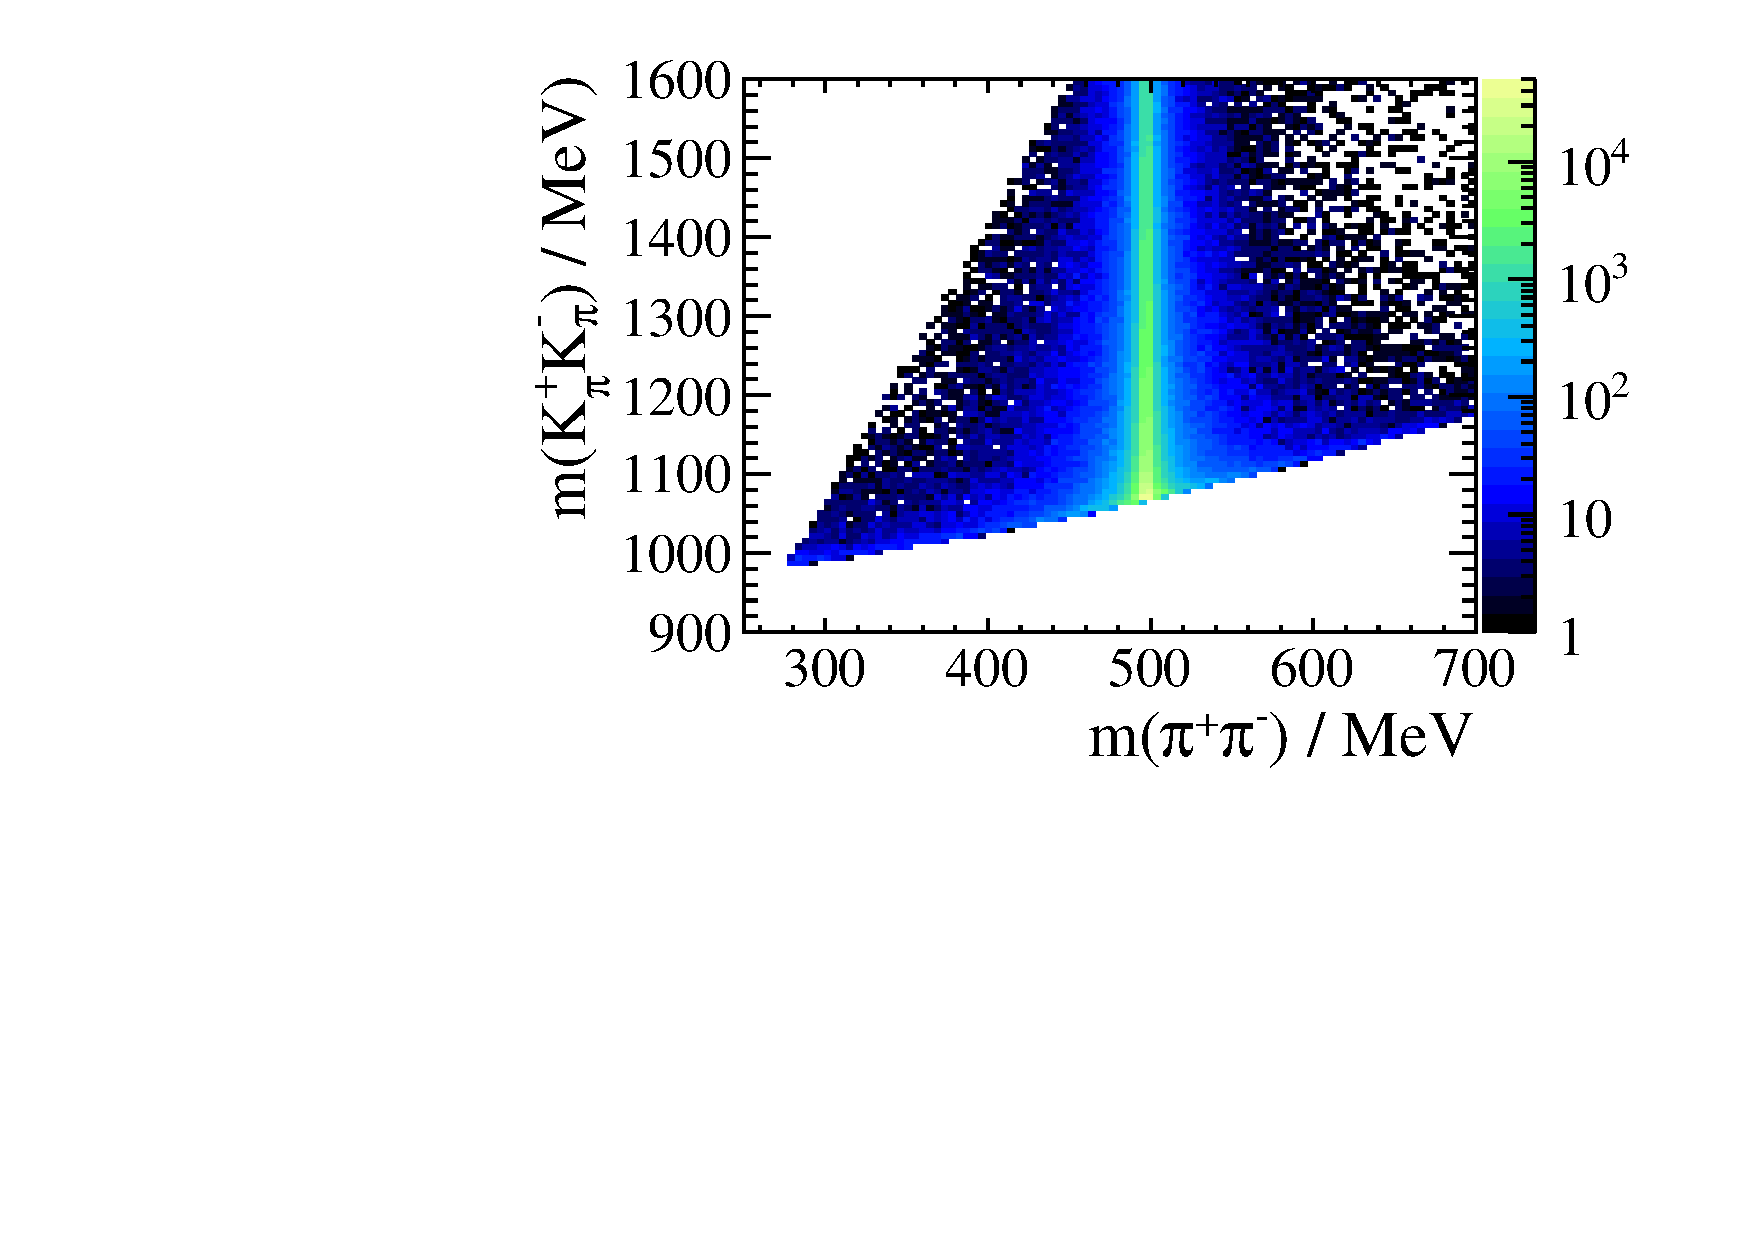
\includegraphics[width=0.48\textwidth]{gen_kk_pipi}
    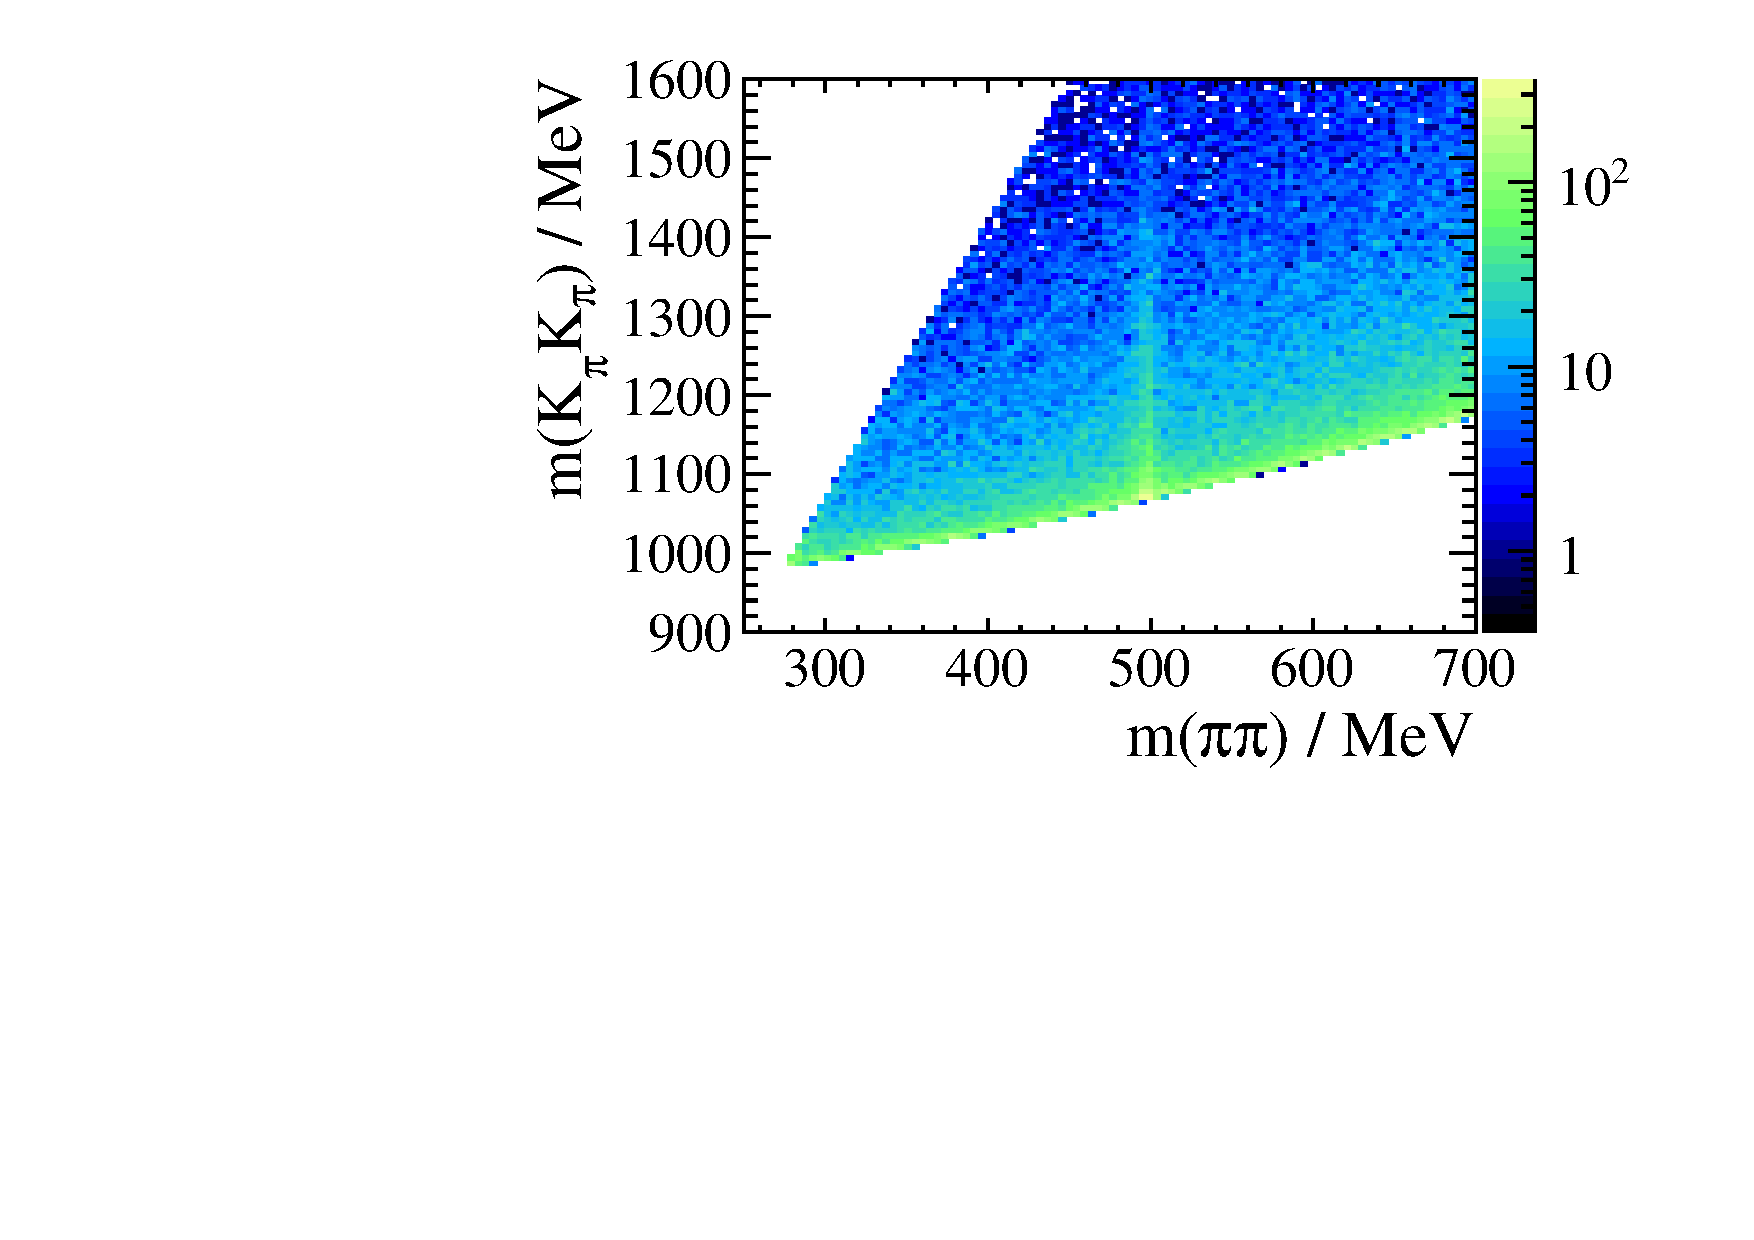
\includegraphics[width=0.48\textwidth]{data_kk_pipi}\\
    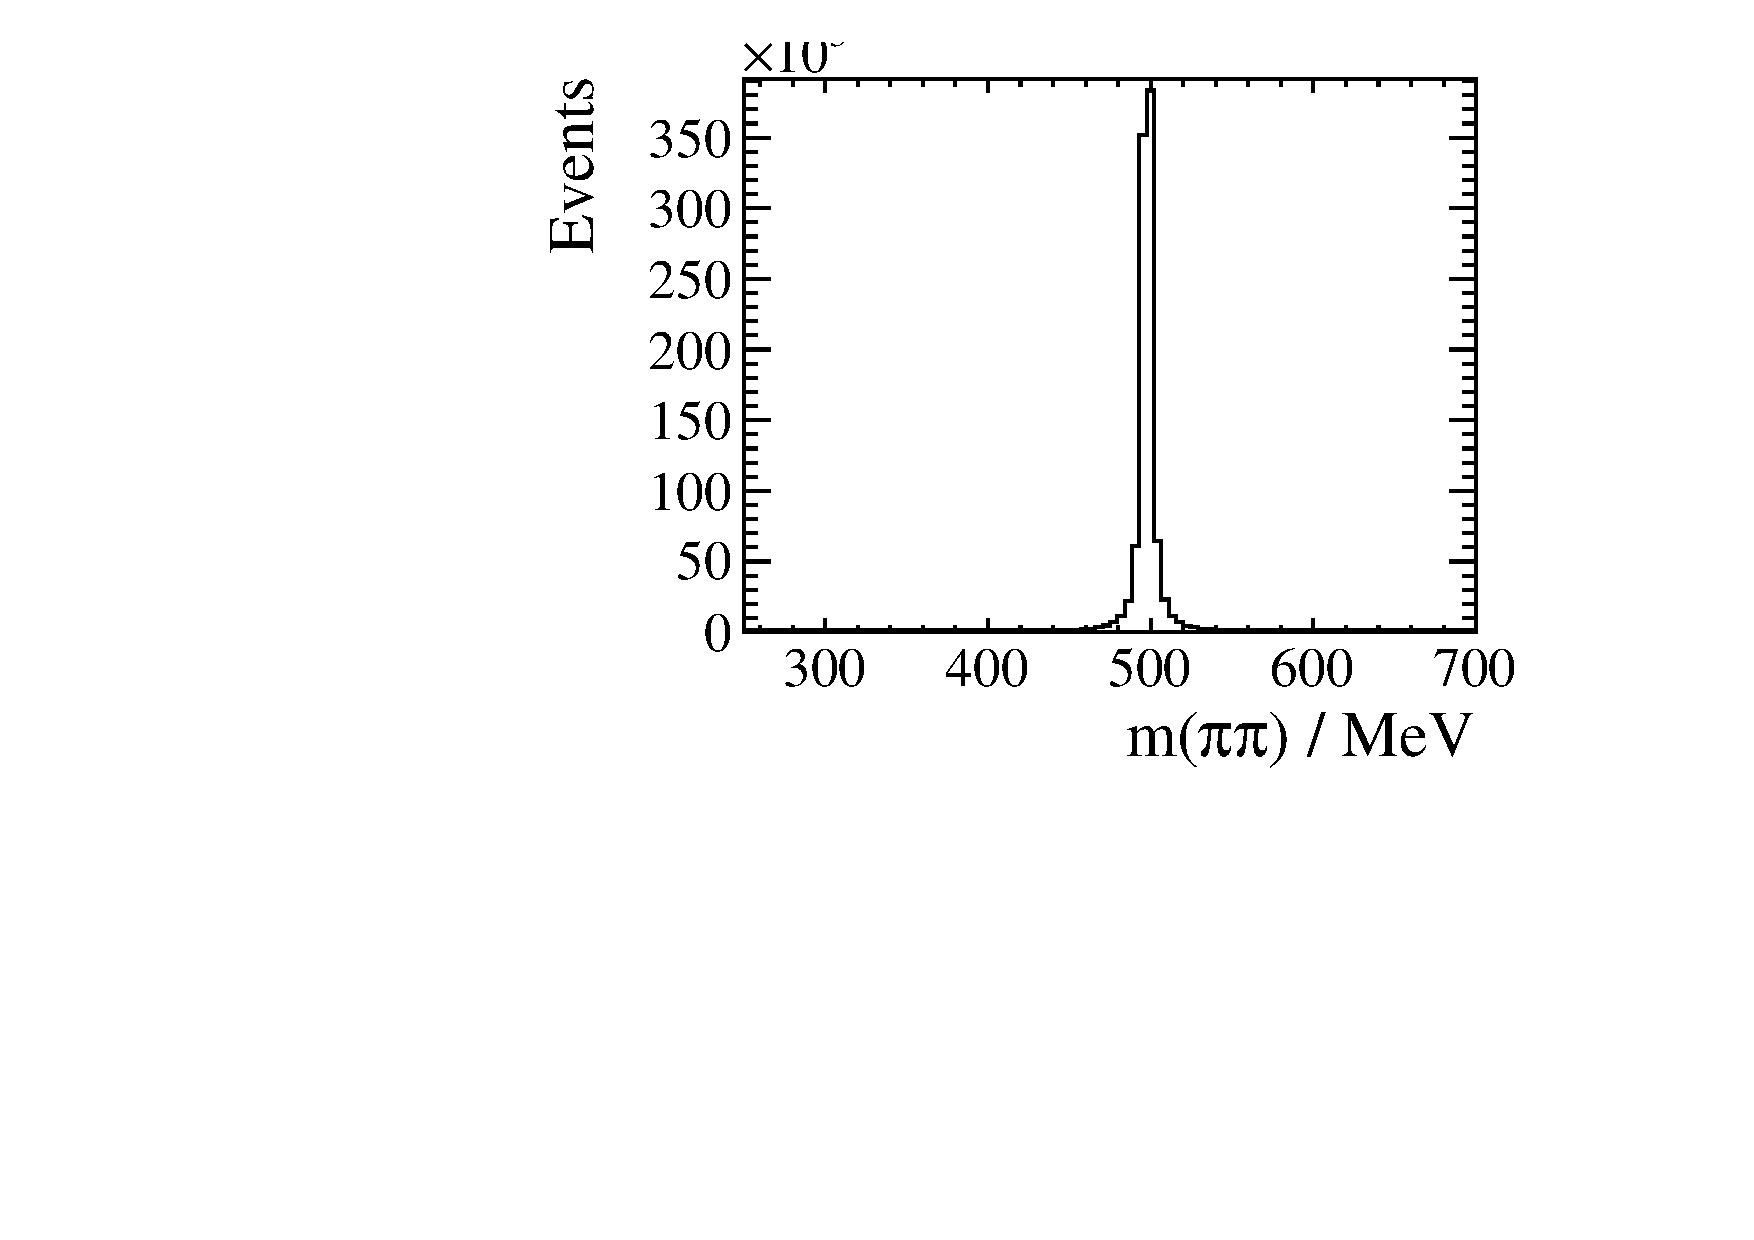
\includegraphics[width=0.48\textwidth]{gen_pipi}
    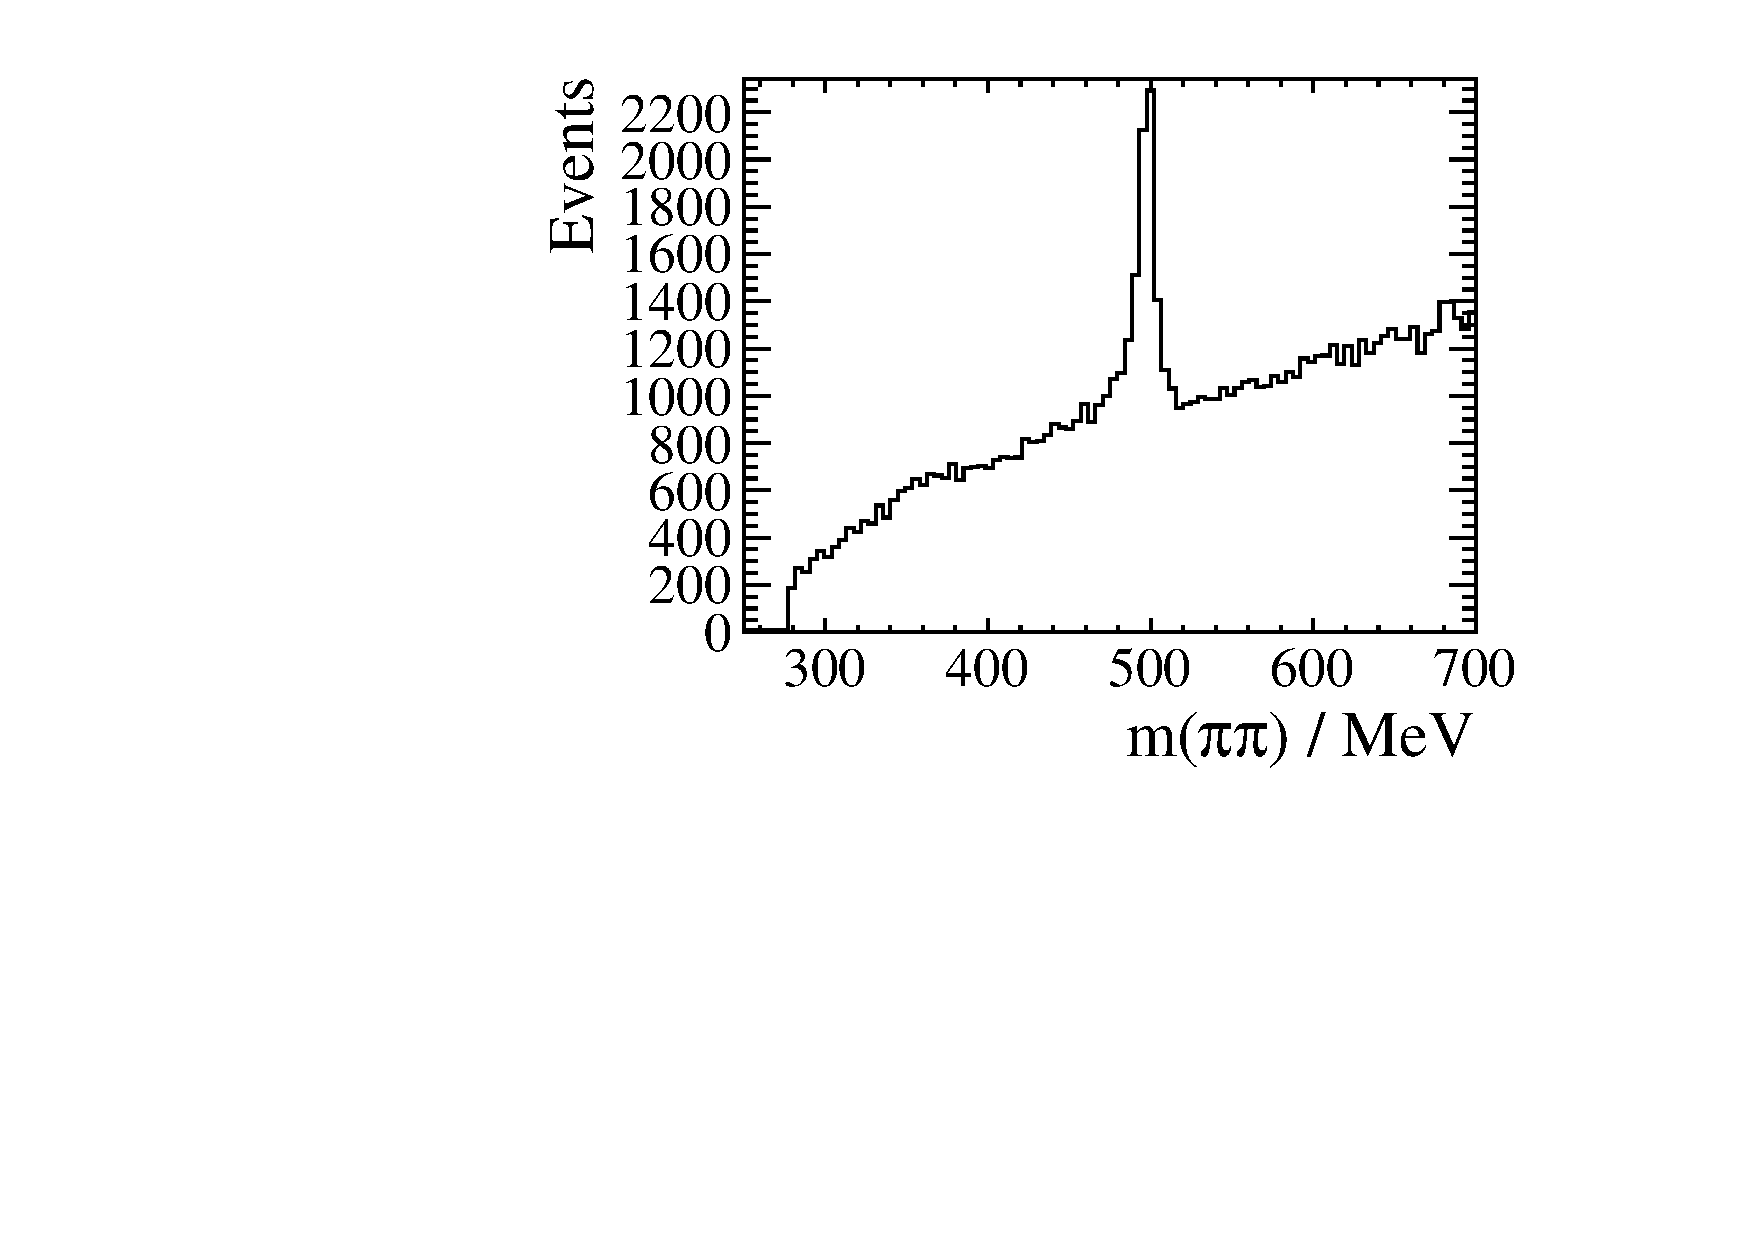
\includegraphics[width=0.48\textwidth]{data_pipi}\\
    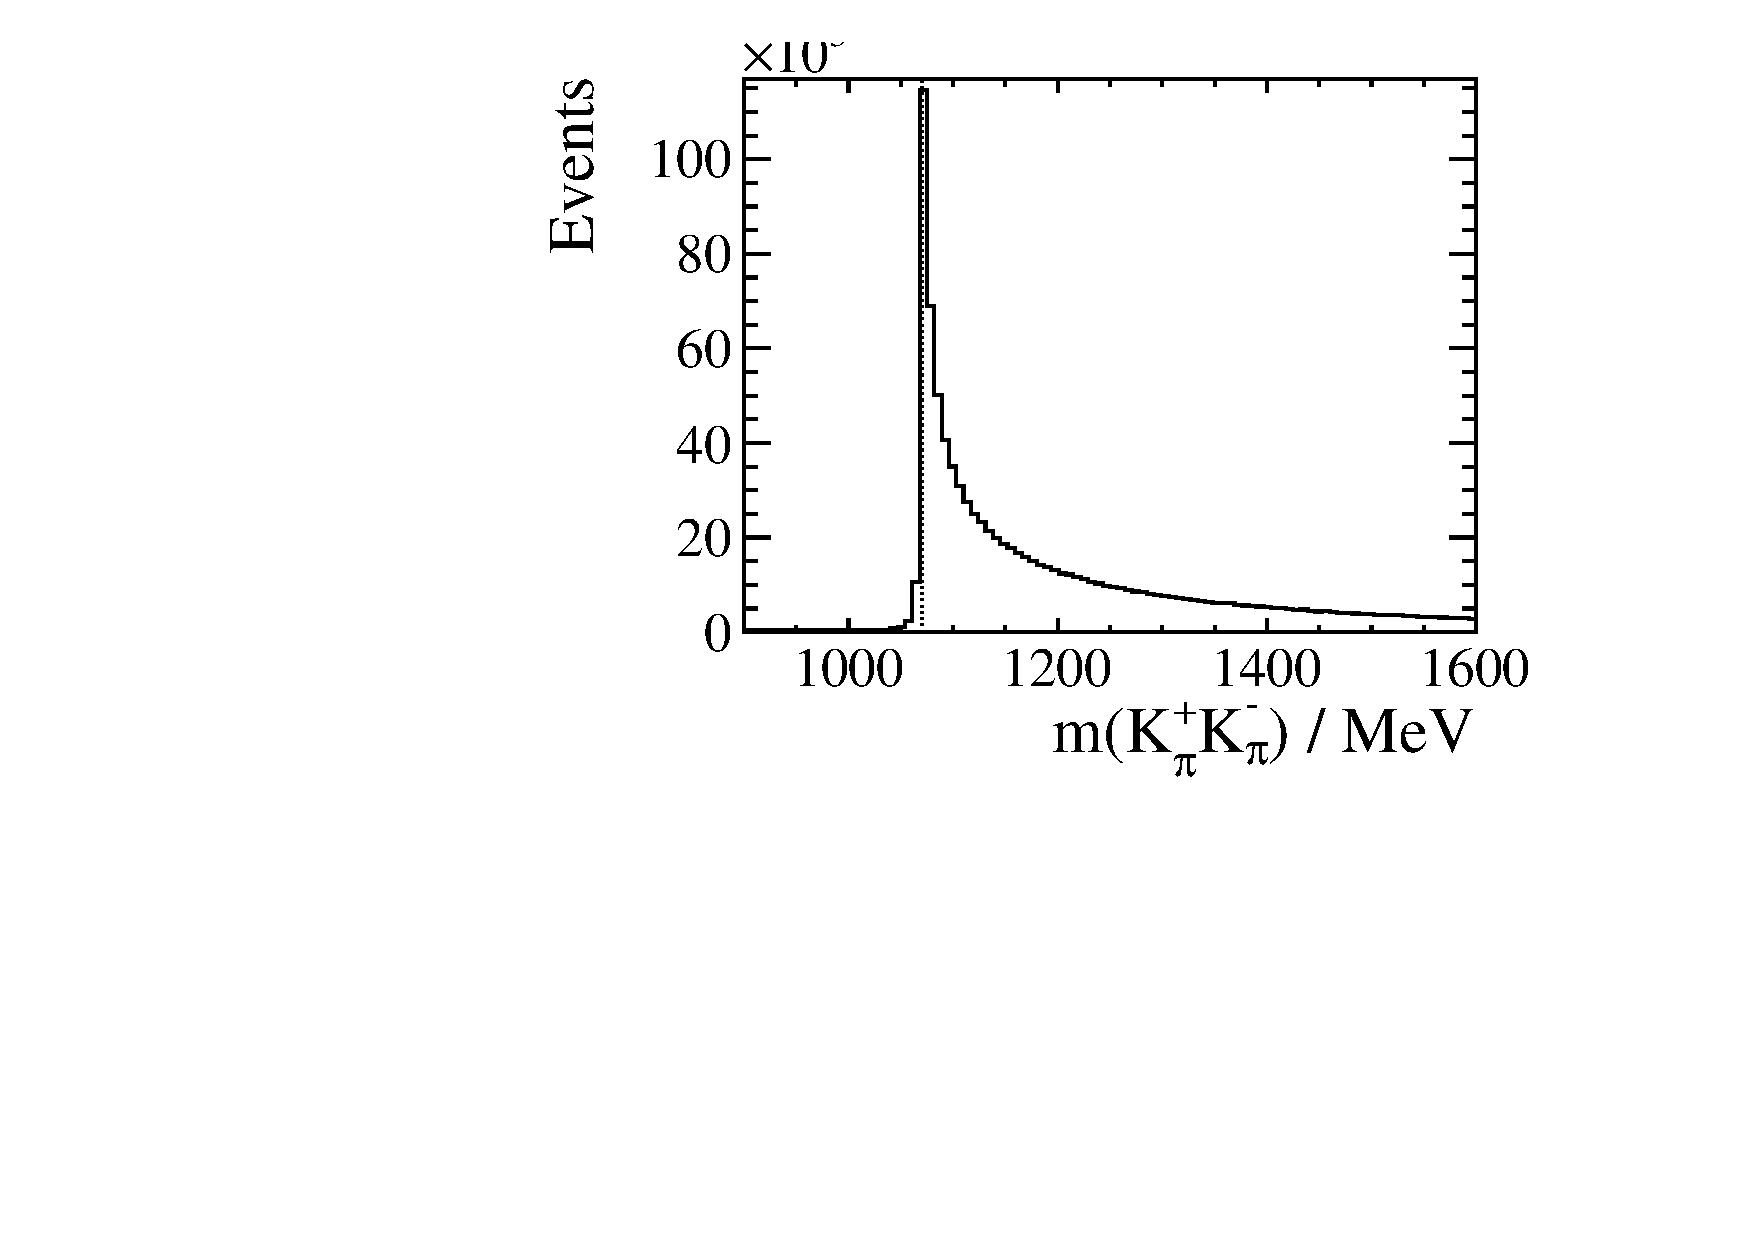
\includegraphics[width=0.48\textwidth]{gen_kk}
    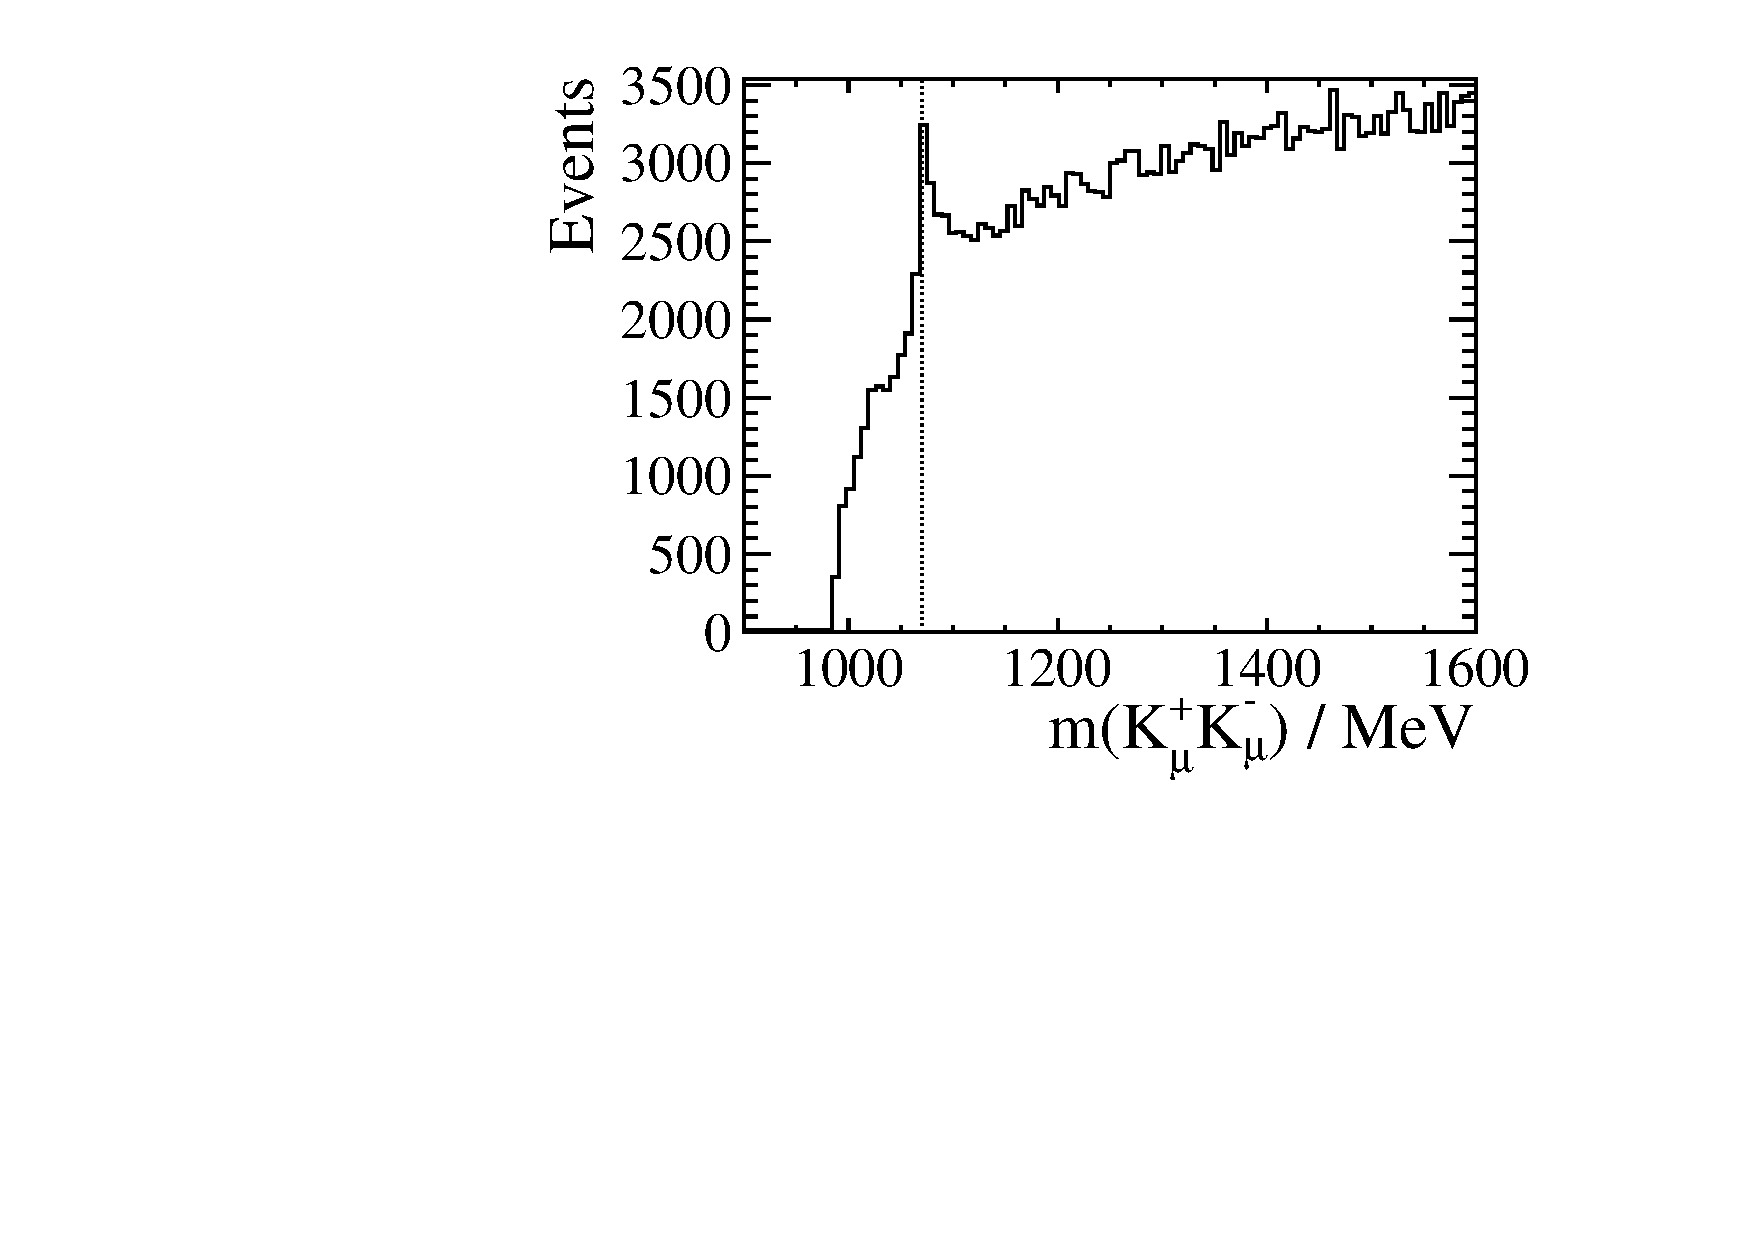
\includegraphics[width=0.48\textwidth]{data_kk}
    \caption[Analysis of the \decay{\KS}{\pipi} background under the \kk mass hypothesis]
    {
      A comparison of \decay{\KS}{\pi\pi} under different mass hypotheses, for
      (left) simulated events, and
      (right) events from data.
      The (top) plots show the two dimensional distributions of the invariant mass distributions of
      a \pipi pair and the same candidates in the \kk mass hypothesis, the (middle) and (bottom)
      plots show the projections.
      Vertical lines in the lower plots indicate $1072\mev$.
    }
    \label{fig:db:x1070:2d}
  \end{center}
\end{figure}


